\section{Durchführung}
Der Versuchsaufbau zur Messung der Wellenlänge als auch
zur Bestimmung des Brechungsindex von Luft ist in Abbildung \ref{abb:3}
dargestellt.
\begin{figure}[H]
  \centering
  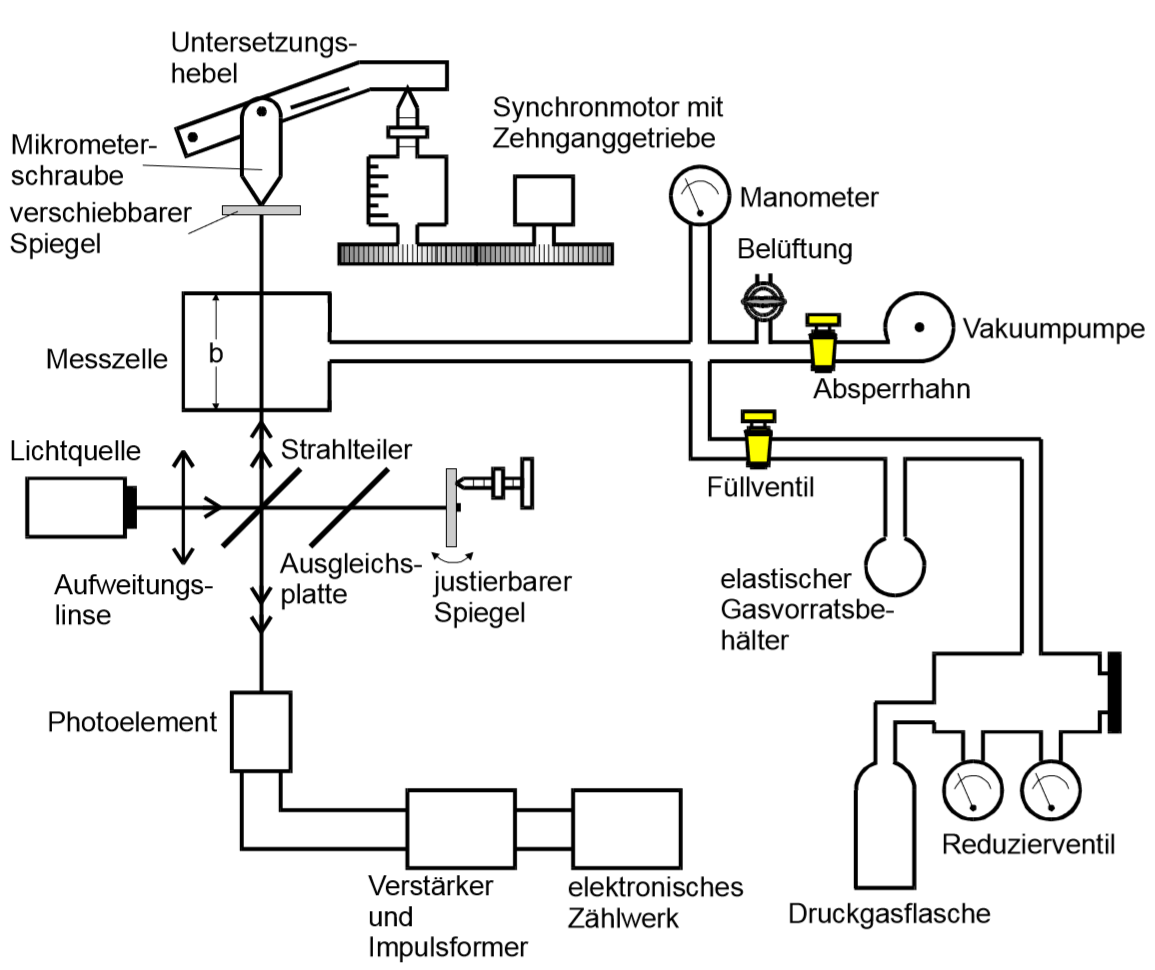
\includegraphics[width=\textwidth]{content/Aufbau3.png}
  \caption{Aufbau zur Bestimmung von Wellenlänge und Brechungsindex.\cite{1}}
  \label{abb:3}
\end{figure}
Bevor die Messung beginnt, wird zunächst das Michelson-Interferometer justiert.
Dazu wird mithilfe einer Mattscheibe vor dem Detektor $D$ die Strahlen aufgefangen.
Mit dem verstellbaren Spiegel wird versucht, dass die Strahlen möglichst aufeinander liegen.
Um die Interferenz besser sehen zu können wird vor dem Laser eine Sammellinse platziert.
Der Detektor wird anschließend noch auf die richtige Höhe gebracht, sodass eine Zählung
der Helligkeitsmaxima möglich ist.
Nun wird ein verschiebbarer Spiegel mithilfe eines Motors um Mikrometer verschoben.
Dabei ist zu beachten, dass der Spiegel sich nicht zu schnell bewegt, da sonst der
Detektor nicht alle Helligkeitsmaxima aufzeichnen kann.
Es wird nun die Länge $d_0$ aufgezeichnet sowie die Anzahl der Maxima. Um möglichst
genau die Wellenlänge des Lasers bestimmen zu können wird der Versuch achtmal durchgeführt.
Um den Brechungsindex von Luft zu messen, wird in der Messzelle ein Unterdruck
erzeugt. Die Messzelle hat eine Länge von $b = \SI{50}{\milli\meter}$.
Dabei werden die Spiegel nicht verstellt. Beim wieder einlassen der Luft entstehen Helligkeitsmaxima
welche wieder von dem Detektor gezählt werden.
